\setcounter{page}{1} %设置起始页面
\section{最初的开始}
\songti
\subsection{第一个脚印}

\subsubsection{小小1}
\subsubsection{小小2}

\subsection{第二个脚印}

\subsubsection{表格}
准确率和召回率指标表格,如表\ref{f1score}所示
\begin{table}[H]
\centering
\begin{tabular}{|ll|ll|}
\hline
\multicolumn{2}{|l|}{\multirow{2}{*}{}}       & \multicolumn{2}{c|}{实际}      \\ \cline{3-4} 
\multicolumn{2}{|l|}{}                        & \multicolumn{1}{l|}{1}  & 0  \\ \hline
\multicolumn{1}{|r|}{\multirow{2}{*}{预测}} & 1 & \multicolumn{1}{l|}{TP} & FP \\ \cline{2-4} 
\multicolumn{1}{|r|}{}                    & 0 & \multicolumn{1}{l|}{FN} & TN \\ \hline
\end{tabular}
% 表格标注
\caption{召回率和精度}
\label{f1score}
\end{table}

\subsubsection{图片}
这是一张远距离连接装置的图片,如图\ref{fig_la}所示:
\begin{figure}[H]
	\centering
	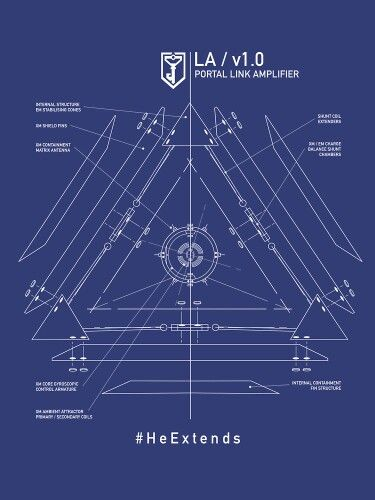
\includegraphics[width=2in]{figures/la.jpg}
	\caption{远距离连接装置}
	\label{fig_la}
\end{figure}

\subsection{引用}

这篇文章参考了 Donald E. Knuth 大佬写的书\cite{1989The}